\documentclass[a4paper,10pt,oneside]{article}
\usepackage[polutonikogreek,italian]{babel}
\usepackage[utf8x]{inputenc}
\usepackage{amsmath}
\usepackage{amsthm}
\usepackage{amssymb}
\usepackage{amscd}
\usepackage{setspace}
\usepackage{graphicx}
\usepackage{float}
\usepackage{array}
\usepackage{rotating}
\usepackage[small]{caption}
\usepackage{lscape}
\usepackage{fancybox}
\usepackage{booktabs}
%\usepackage[noanswer]{exercise}
\parindent0ex 
\renewcommand{\fboxsep}{0.5cm}
\newtheorem{regola}{Regola}
\usepackage{hyperref}
\renewcommand{\textfraction}{0.05}
\renewcommand{\topfraction}{0.95}
\renewcommand{\bottomfraction}{0.95}
\renewcommand{\floatpagefraction}{0.35}
%\renewcommand{\ExerciseName}{Esercizio}
%\renewcommand{\ExerciseListName}{Es}
\setcounter{totalnumber}{5}
\restylefloat{figure}
\newlength{\drop}
\begin{document}
\begin{center}
\begin{doublespace}
 {\huge \textbf{Laboratorio di cinematica $1,2$-dimensionale}}
\end{doublespace}
\end{center}

\begin{abstract}
 La cinematica, dal greco \textgreek{κινεῖν} (velocità), è quella branca della fisica che si occupa di descrivere il moto degli oggetti. In questo laboratorio tratteremo della relazione spazio-tempo per corpi in moto lungo traiettorie bidimensionali e unidimensionali
\end{abstract}


\vspace{1.5cm}

Per gli esperimenti sui moti unidimensionali utilizzeremo la guidovia a cuscino d'aria del laboratorio del liceo, figura [\ref{fig:guidovia_cuscino}].

\begin{figure}[H]
 \centering
 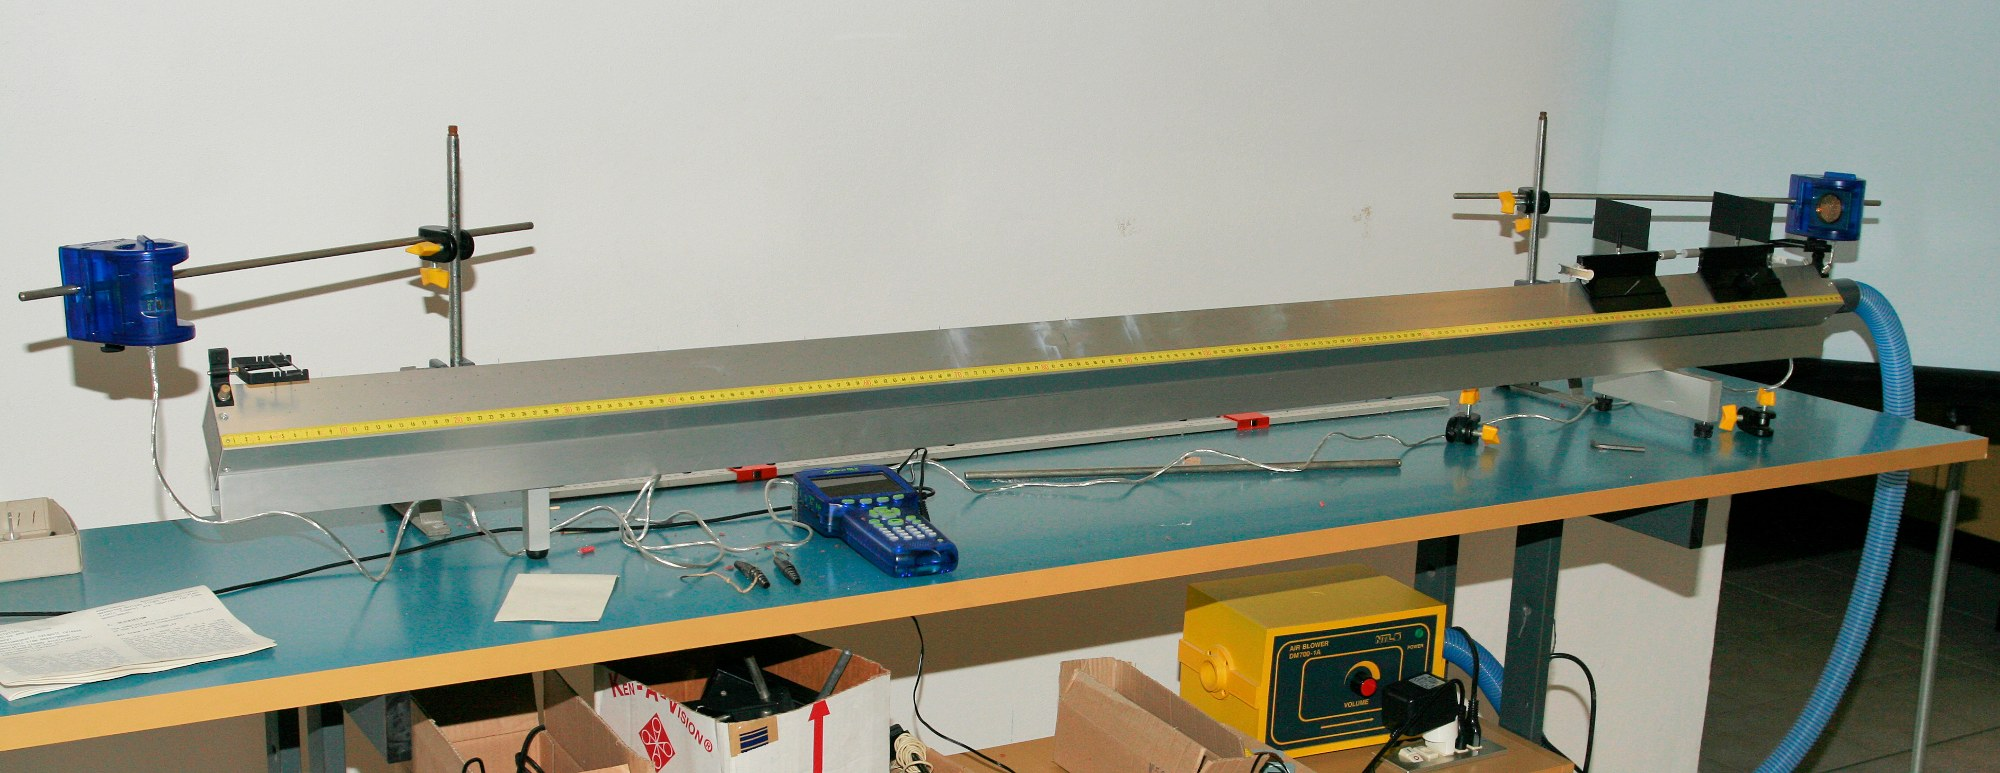
\includegraphics[width=0.8\textwidth]{./Immagini/guidovia.jpg}
 % guidovia.png: 3774x1458 pixel, 72dpi, 133.12x51.43 cm, bb=
 \caption{Guidovia a cuscino d'aria con sensori di posizione montati}
 \label{fig:guidovia_cuscino}
\end{figure}

La posizione dei carrelli lungo la guidovia verrà  campionata con i sensori di posizione ultrasonici  \textsl{CI-6742}, figura [\ref{fig:Pasco_sensore1}], della Pasco che verranno montati durante l'esperienza tramite della staffe. In rete è disponibile un \emph{datasheet} completo dei sensori riportante tutte le loro caratteristiche tecniche\footnote{Come esercizio cercate il file pdf con le caratteristiche dei sensori di posizione che potrete poi citare nelle vostre relazioni}.

\begin{figure}[H]
 \centering
 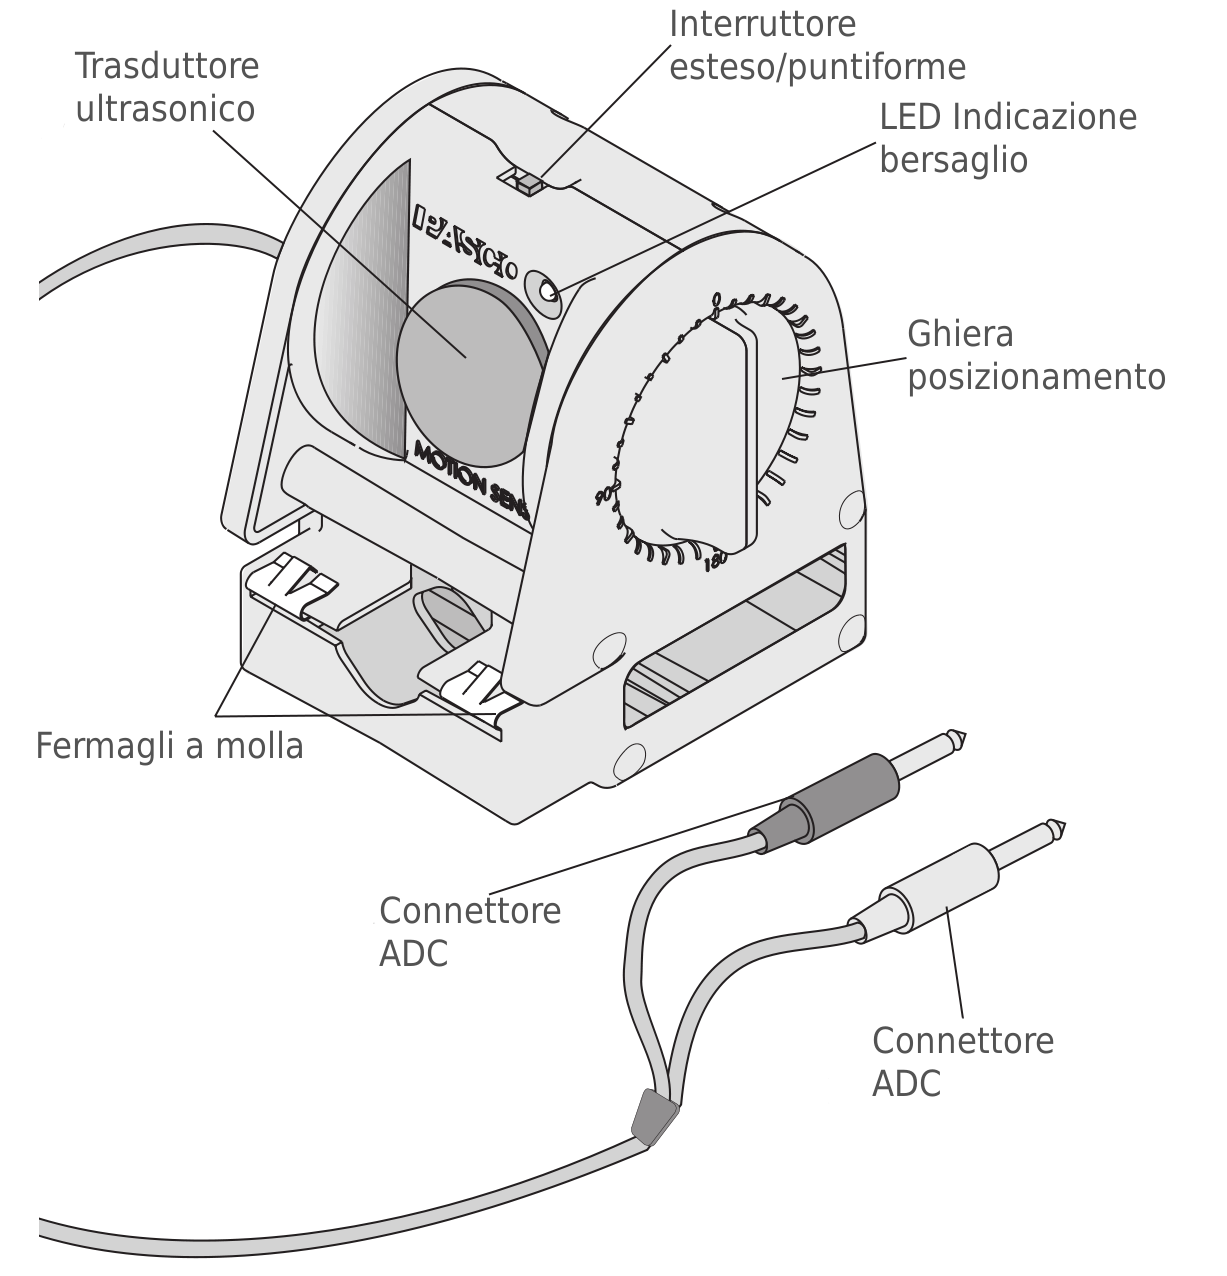
\includegraphics[width=0.5\textwidth]{./Immagini/sensore_moto_pasco.png}
 % sensore_moto_Pasco.png: 1227x1276 pixel, 300dpi, 10.39x10.80 cm, bb=
 \caption{Sensore di posizione Pasco, disegno tratto dal datasheet della strumentazione}
 \label{fig:Pasco_sensore1}
\end{figure}
Per studiare  i moti bidimensionali utilizzeremo, invece, dei piccoli cannoni ad elastico con i quali lanceremo dei proiettili il cui moto verrà ripreso e quindi analizzato tramite il programma Tracker.
\begin{figure}[H]
 \centering
 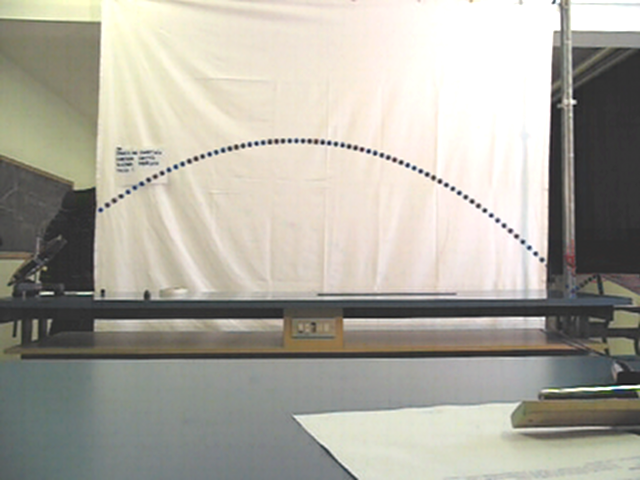
\includegraphics[width=0.7\textwidth]{./Immagini/traiettoria.png}
 % traiettoria.png: 640x480 pixel, 72dpi, 22.57x16.93 cm, bb=0 0 640 480
 \caption{Traiettoria del proiettile estratta da un filmato a $240\ Hz$ ripreso durante il secondo laboratorio di cinematica anno scolastico 2010/2011}
 \label{fig:traiettoria_1}
\end{figure}


\section*{Esercizio con la guidovia a cuscino d'aria}

\emph{Un treno passa davanti ad un passaggio a livello. La locomotiva transita in $T_1$ secondi l'ultimo vagone transita in $T_2$ secondi. Sapendo che il treno è composto di $n$ elementi della stessa lunghezza $L$, determinarne l'accelerazione nell'ipotesi che questa sia uniforme.}\footnote{Esercizio proposto dal prof. Marco Clocchiatti dell'Isis Paschini di Tolmezzo}.

Possiamo rispondere, in via sperimentale, al precedente esercizio misurando con i sensori di posizione della Pasco l'accelerazione del convoglio, che in laboratorio sarà rappresentato da due slitte collegate fra loro da un filo. La misura diretta è molto semplice però non ci insegna nulla di particolarmente interessante, per questo motivo tramite una fotocellula misureremo il tempo di transito del primo e dell'ultimo ``convoglio'' del nostro ``treno'' e quindi dedurremo un'espressione analitica dell'accelerazione in funzione  dei parametri del problema:
\begin{equation}
 a=f(L,T_1,T_2,n)
\end{equation}
La soluzione analitica  è lasciata a voi come utile esercizio di cinematica unidimensionale, la migliore tra quelle proposte verrà a tempo debito pubblicata all'indirizzo \url{http://cartan.e-moka.net}.

\subsection*{Stima degli errori}
Tutti i dati raccolti in laboratorio saranno affetti da errori sperimentali per questo motivo le grandezze derivate che calcoleremo (velocità ed accelerazione) presenteranno  un'incertezza. Al fine di valutarne la significatività sarà necessario determinare come l'incertezza sulle grandezze misurate si rifletta su quelle calcolate. In questi semplici esperimenti le uniche operazioni coinvolte saranno somme, prodotti e quozienti questo ci permette di calcolare l'errore con relativa facilità. Seguiremo le due regole:

\begin{regola}\footnote{Se le incertezze sulle misure sono indipendenti e casuali allora possiamo utilizzare una stima più accurata per l'errore nota come somma in quadratura}

Se delle grandezze $x_1,x_2,x_3,x_4\ldots$ sono misurate con incertezze $\delta x_1,\delta x_2,\delta x_3, \delta x_4\ldots$ ed i valori sono utilizzati per calcolare una grandezza derivata

\begin{equation*}
y=x_1+x_2+x_3+x_4\ldots
\end{equation*}
l'errore massimo su $y$ che chiameremo $\delta y$ sarà dato da:
\begin{equation*}
 \delta y\approx\delta x_1+\delta x_2+\delta x_3+\delta x_4+\ldots
\end{equation*}
\end{regola}

\begin{regola}

Se delle grandezze $x_1,x_2,x_3,x_4\ldots$ sono misurate con incertezze $\delta x_1,\delta x_2,\delta x_3,\delta x_4\ldots$ ed i valori sono utilizzati per calcolare una grandezza derivata:
\begin{equation*}
 y=\frac{x_1 x_2\ldots}{x_3 x_4\ldots}
\end{equation*}
allora l'errore relativo sulla grandezza derivata $y$ sarà la somma degli errori relativi delle misure:
\begin{equation*}
 \frac{\delta y}{|y|}\approx \frac{\delta x_1}{|x_1|}+\frac{\delta x_2}{|x_2|} +\frac{\delta x_3}{|x_3|}+\frac{\delta x_4}{|x_4|}+\ldots
\end{equation*}

\end{regola}

Utilizzando un foglio di calcolo (ad esempio Libre Office Calc) determinate l'errore che affligge velocità ed accelerazione misurate con gli strumenti Pasco. Chi volesse approfondire può consultare il manuale introduttivo sul calcolo degli errori  [\cite{taylor}].

\section*{Esportazione dei dati da Pasco Data Studio}
Il programma Data Studio, installato nei computer del laboratorio di fisica, ci permette di acquisire le misurazioni dai sensori di posizione e di effettuare le prime analisi sui dati figura [\ref{fig:pasco_dati1}].
\begin{figure}[H]
 \centering
 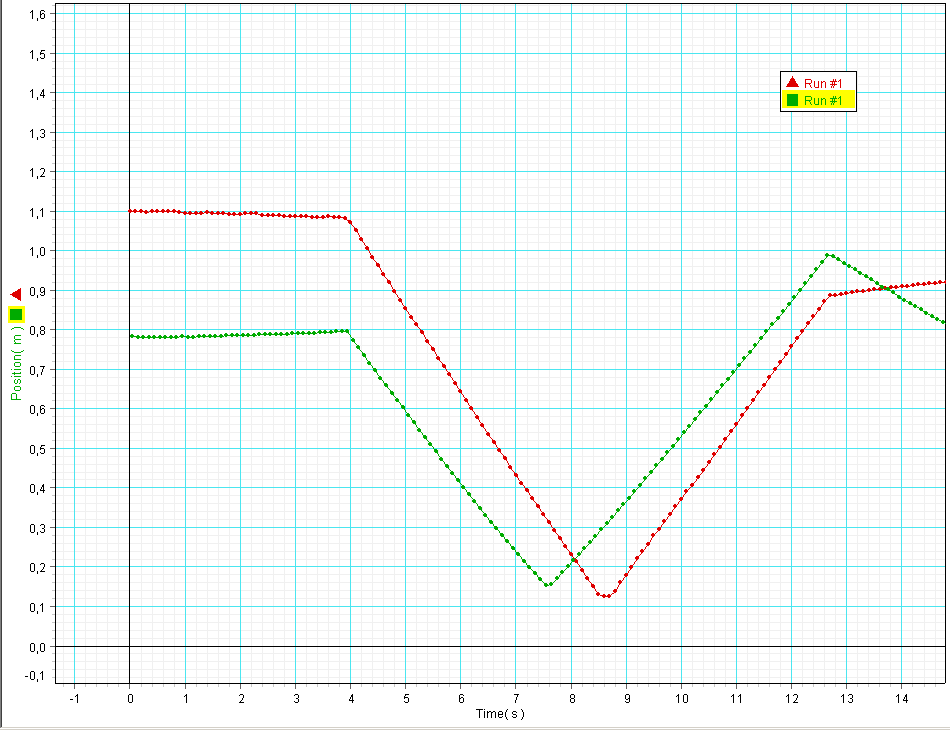
\includegraphics[width=0.7\textwidth]{./Immagini/pasco2.png}
 % pasco2.png: 1152x867 pixel, 96dpi, 30.48x22.94 cm, bb=
 \caption{Serie dai misure acquisite tramite Pasco Datastudio}
 \label{fig:pasco_dati1}
\end{figure}

Il programma permette l'esportazione dei dati acquisiti  in formato testuale per una successiva analisi manuale o tramite altri software dedicati al calcolo numerico. La procedura di esportazione è molto semplice, dal menu \textsl{File} selezionate \textsl{Esporta dati\ldots} e scegliete quindi l'insieme di misure da esportare figura [\ref{fig:pasco_export}].
\begin{figure}
 \centering
 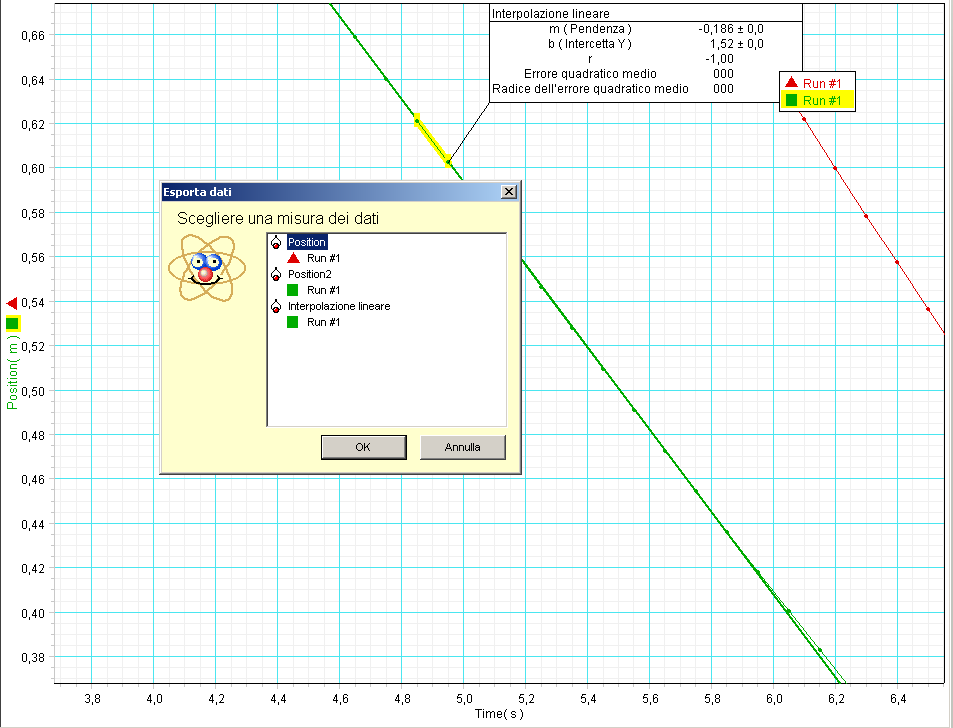
\includegraphics[width=0.7\textwidth]{./Immagini/pasco3.png}
 \caption{Esportazione dei dati da Pasco Data Studio}
 \label{fig:pasco_export}
\end{figure}

I dati saranno esportati in un file di testo utilizzabile poi da tutti i programmi di analisi numerica:
\begin{verbatim}
Position, Run #1
Time ( s )	Position ( m )
0,0032	1,100
0,1032	1,099
0,2032	1,100
0,3032	1,096
0,4032	1,099
0,5032	1,099
0,6032	1,099
0,7032	1,099
\end{verbatim}

\section*{Moto parabolico}

Per studiare il moto di un proiettile utilizzeremo un cannone ad elastico come in figura [\ref{fig:cannone1}]
\begin{figure}[H]
 \centering
 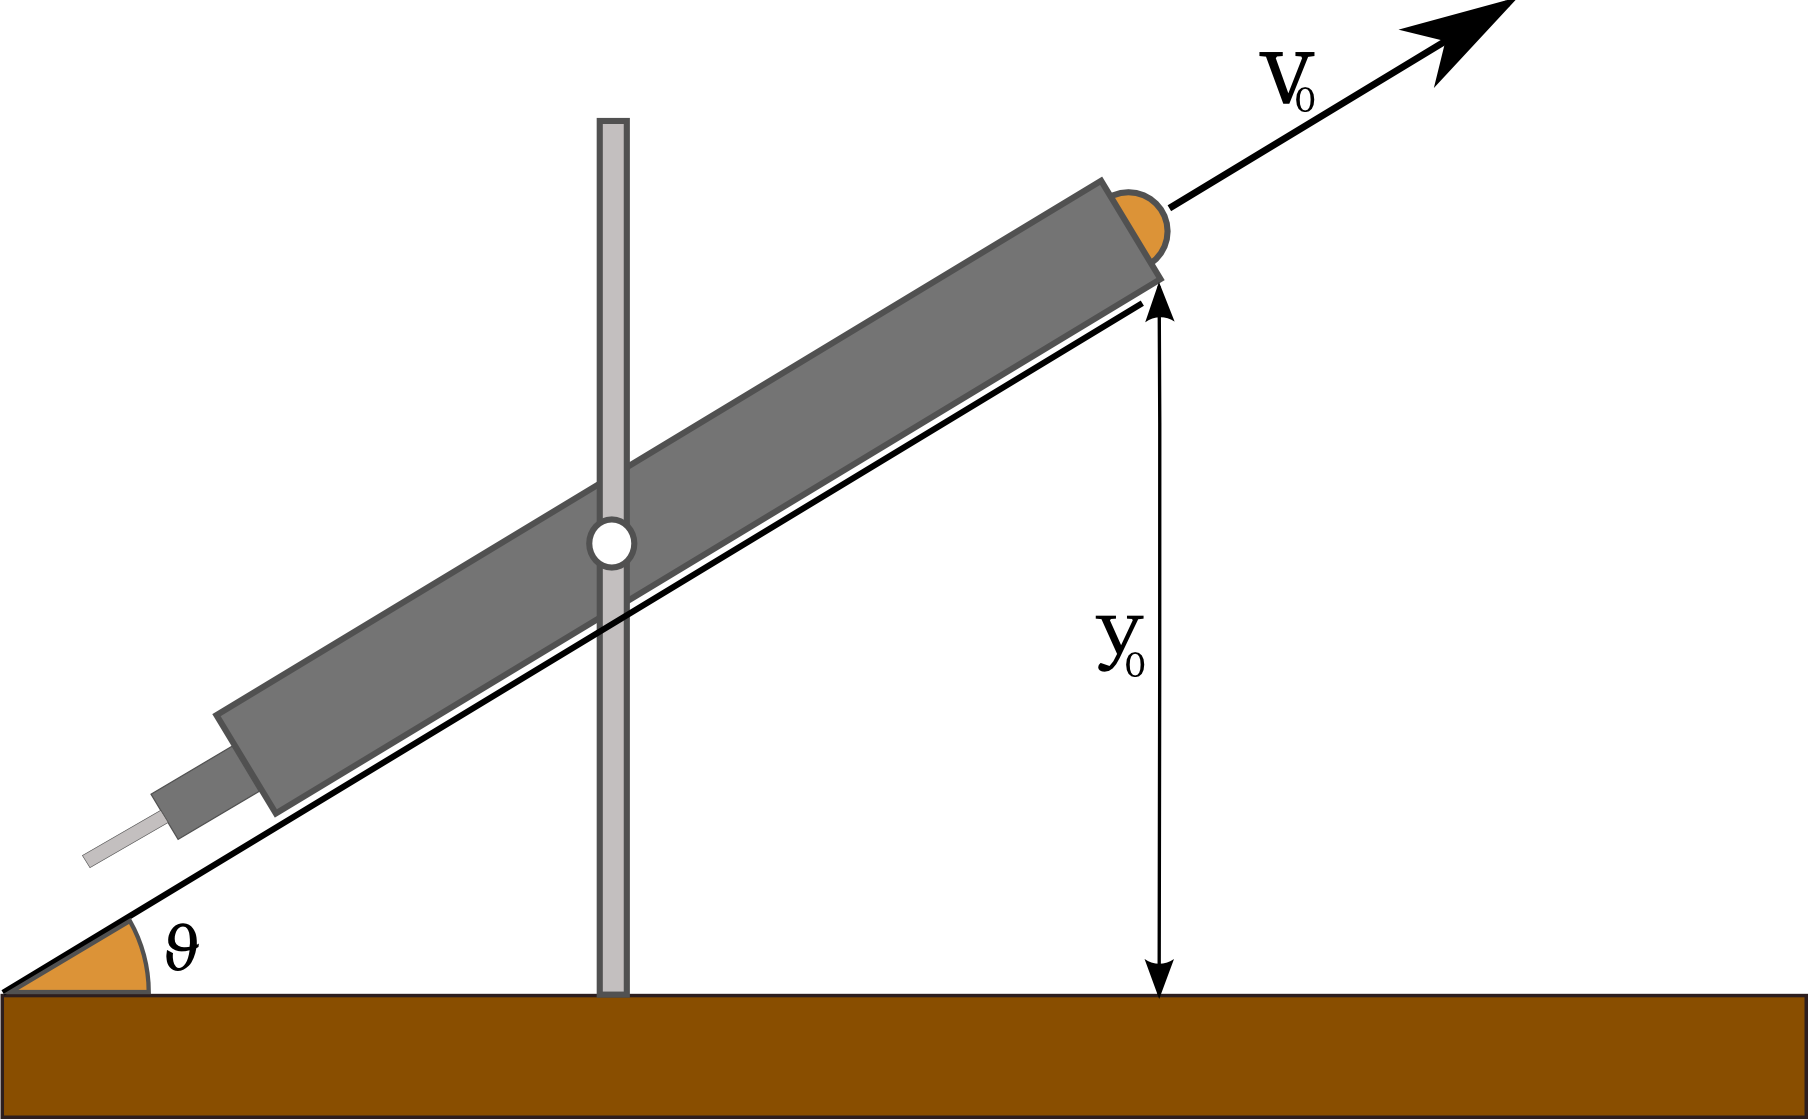
\includegraphics[width=0.7\textwidth]{./Immagini/cannone.png}
 % cannone.png: 1808x1119 pixel, 500dpi, 9.19x5.69 cm, bb=
 \caption{Cannone ad elastico montato in laboratorio}
 \label{fig:cannone1}
\end{figure}
Durante gli esperimenti la bocca del cannone si troverà ad una quota $y_0$, l'inclinazione del tubo di lancio sarà $\theta$ e la velocità iniziale del proiettile sarà $v_0$. Le componenti della velocità $\mathbf{v}(t)$ saranno:
\begin{align}
 v_x(t)&=v_0\cos \theta\\
 v_y(t)&=v_0\sin\theta -gt
\end{align}
dove $g$ è l'accelerazione di gravità. Le componenti dello spostamento saranno:
\begin{align}\label{posizione}
 x(t)&=v_0t\cos\theta\\
 y(t)&=y_0+v_0t\sin \theta -\frac{1}{2} g t^2
\end{align}

dove si è presupposto che la bocca del cannone si trovi alle coordinate $x=0$ e $y=y_0$. Dalle [\ref{posizione}] possiamo ricavare facilmente la distanza $L$ dalla bocca del cannone ad un istante $t$:
\begin{equation}
 L(t)=\sqrt{(v_0 t\cos\theta )^2+(v_0t \sin \theta-\frac 1 2 g t^2)^2}
\end{equation}

e la gittata in  funzione dell'angolo $\theta$:
\begin{equation}
 g(\theta)=v_0\cos \theta\frac{v_0\sin\theta+\sqrt{v^2\sin^2\theta+2 y_0 g}}{g}
\end{equation}
avremo gittata massima per un angolo $\theta$:
\begin{equation}
 \theta_{max}=\arccos\sqrt{\frac{v_0^2+2gy_0}{2v_0^2+2gy_0}}
\end{equation}

possiamo notare che se $y_0=0$ allora $\theta_{max}=\arccos\frac{1}{\sqrt 2}=\pi/4$ 
\begin{figure}[H]
 \centering
 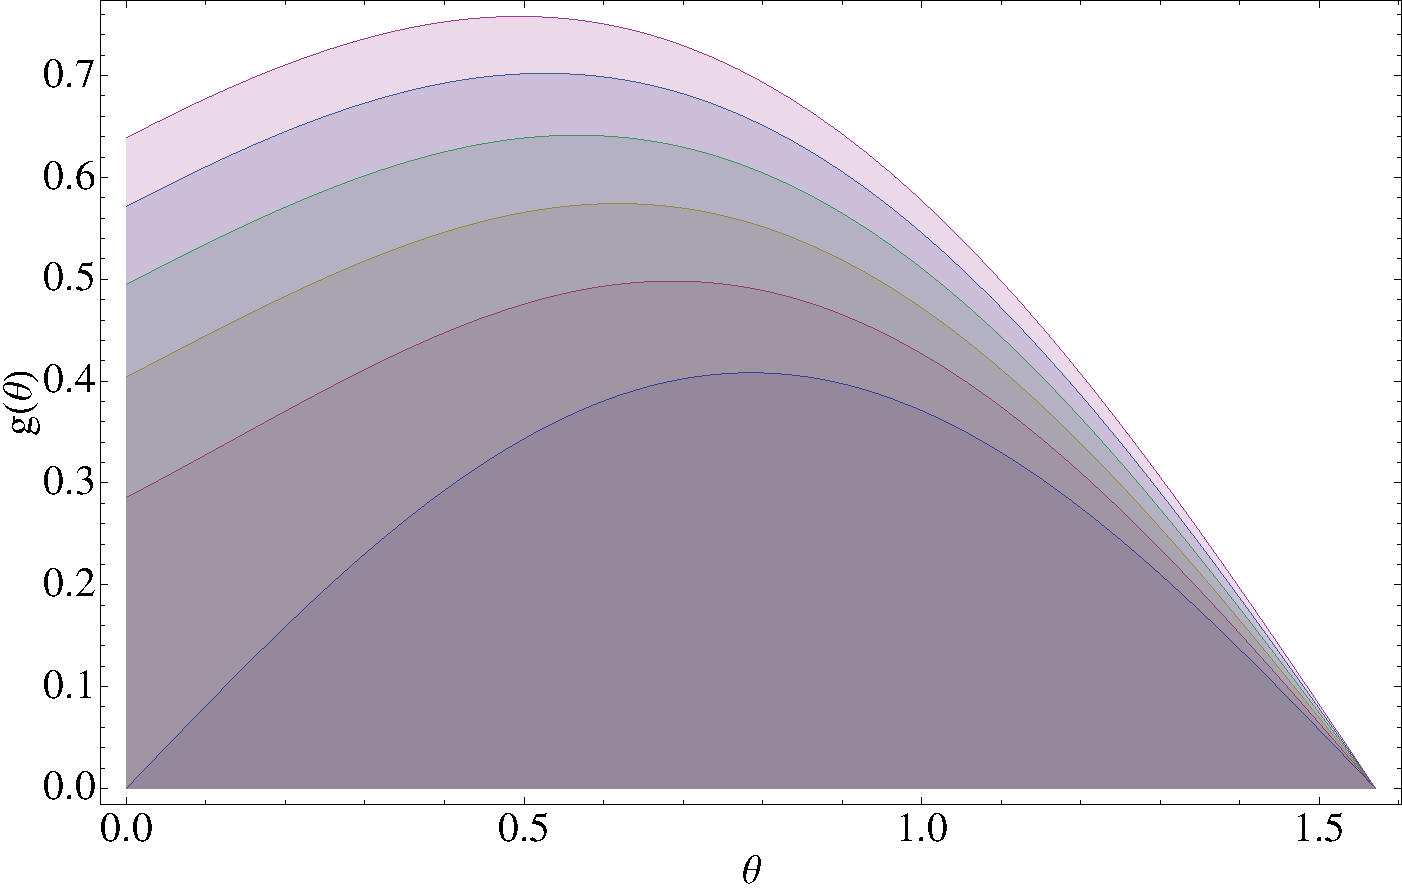
\includegraphics[width=\textwidth]{./Immagini/gittata1.pdf}
 % gittata1.pdf: 673x428 pixel, 72dpi, 23.74x15.10 cm, bb=
 \caption{Gittata in funzione dell'angolo $\theta$ e della posizione iniziale $y_0$ del proiettile. Velocità iniziale $v_0=2ms^{-1}$ e $0\leq y_0\leq 0.5 m$}
 \label{fig:gittata_variazione}
\end{figure}

Tutti calcoli presentati precedentemente si suppongono svolti in assenza di atmosfera, considerando la terra un sistema inerziale e l'accelerazione di gravità costante; per tali motivi i risultati sperimentali si discosteranno dalle previsioni teoriche presentate precedentemente.

\subsection*{Determinazione della gittata}

Per una determinazione sperimentale della relazione che lega la velocità iniziale del proiettile all'inclinazione del cannone e alla quota della bocca del cannone stesso effettueremo svariate prove di lancio per ogni copia di valori $(\theta,y_0)$ e riporteremo i dati in un grafico simile a quello di figura [\ref{fig:gittata_variazione}]. Per minimizzare gli errori sperimentali nel suddetto grafico inseriremo unicamente la media delle misure raccolte per ogni coppia di valori inclinazione-quota iniziale.

\begin{figure}[H]
 \centering
 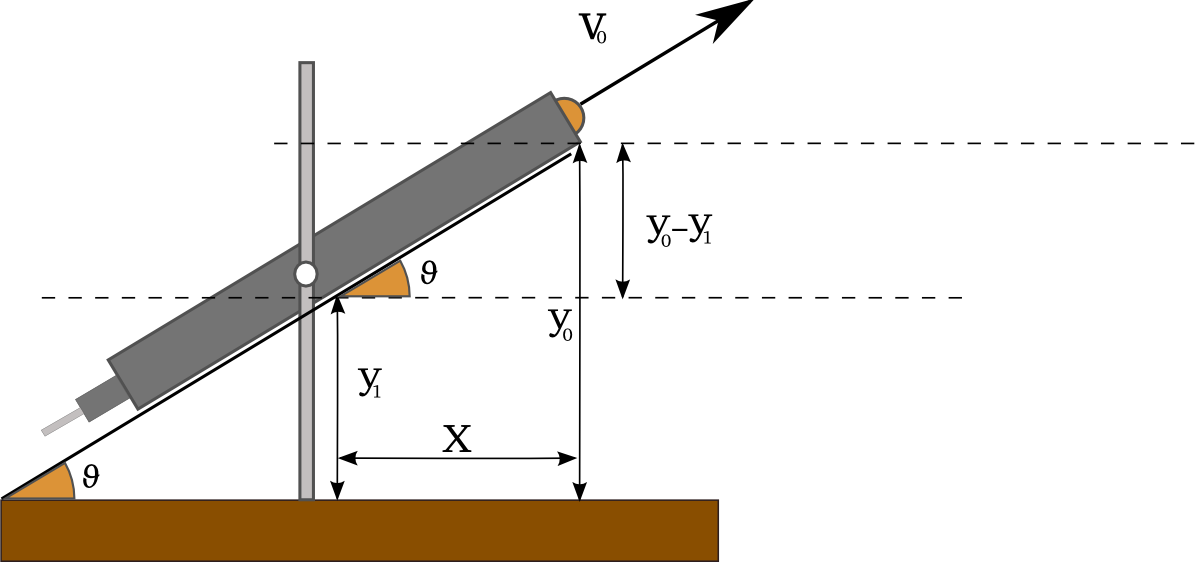
\includegraphics[width=\textwidth]{./Immagini/misura_angolo.png}
 % cannone5.png: 4339x1333 pixel, 500dpi, 22.05x6.77 cm, bb=
 \caption{Misurazione dell'angolo che il cannone forma con l'orizzontale}
 \label{fig:cannone4}
\end{figure}






\subsection*{Traiettoria}

Conoscendo il vettore posizione $\mathbf{r}(t)$ possiamo ricavare la traiettoria della pallina soggetta ad un moto accelerato lungo l'asse verticale ed uno a velocità costante lungo l'asse orizzontale. Siccome le componenti del vettore posizione $\mathbf{r}$ espresse in coordinate cartesiane rappresentano le coordinate della pallina ad un certo istante di tempo $t$ possiamo scrivere il sistema:
\begin{equation}\label{eq:syst1}
\begin{cases}
x=v_0\cos\theta t\\
y=v_0\sin\theta t-\frac{1}{2}gt^2
\end{cases}
\end{equation}
Per ottenere l'equazione della traiettoria dobbiamo cercare una relazione indipendente dal tempo tra le variabili $x$ ed $y$. Dalla [\ref{eq:syst1}] vediamo che è sufficiente ricavare il tempo dalla prima equazione del sistema e sostituirlo nella seconda:
\begin{equation}
\begin{cases}
t=\dfrac{x}{v_0\cos\theta}\\
\\
y=v_0\sin\theta t-\frac{1}{2}gt^2
\end{cases}
\end{equation}
da cui ricaviamo:
\begin{equation}
 y=\tan\theta x-\dfrac{gx^2}{2v_0^2\cos^2\theta}
\end{equation}
ovvero l'equazione di una parabola con la concavità rivolta verso il basso.

Per determinare la traiettoria del proiettile lanciato dal cannone ad elastico,  utilizzeremo una macchina fotografica digitale in grado di riprendere filmati ad alta velocità. 
\begin{figure}[H]
 \centering
 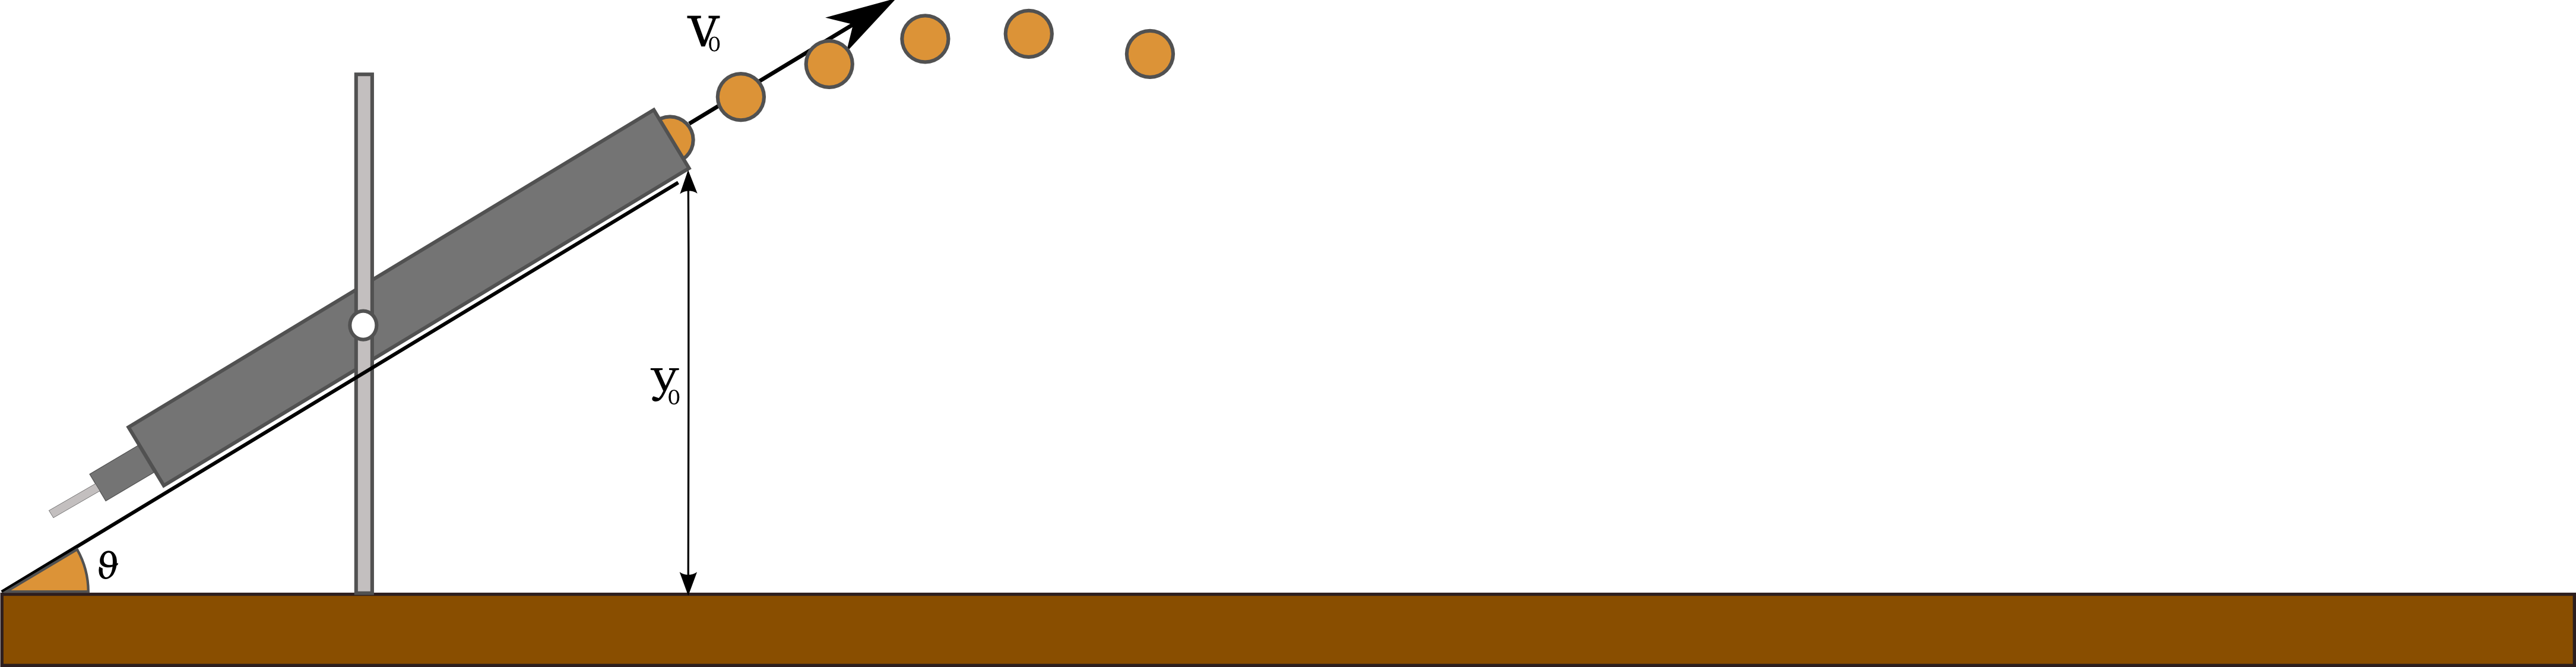
\includegraphics[width=\textwidth]{./Immagini/cannone3.png}
 % cannone3.png: 4339x1123 pixel, 500dpi, 22.05x5.71 cm, bb=
 \caption{La traiettoria sarà determinata misurando le successive posizioni del centro della pallina.}
 \label{fig:cannone3}
\end{figure}
Procederemo nel modo seguente:
\begin{itemize}
 \item Impostiamo la frequenza di campionamento della macchina fotografica (es 240Hz)
\item Riprendiamo il moto per una data estrazione del pistone del cannone.
\item Ripetiamo la ripresa per tre volte (ad allungamento fisso dell'elastico)
\end{itemize}
I filmati dovranno essere poi rielaborati tramite il programma Tracker come visto durante il laboratorio sull'analisi dati. Per meglio visualizzare la traiettoria del proiettile vi consigliamo di effettuare, oltre all'elaborazione con Tracker, anche la sovrapposizione dei fotogrammi con la tecnica esposta durante il laboratorio dello scorso anno\footnote{Potete trovare una guida esemplificativa all'indirizzo \url{http://cartan.e-moka.net/Fisica/Laboratorio/Laboratorio-7-cinematica-bidimensionale}}.





\begin{thebibliography}{}
 \bibitem{taylor} J.R. Taylor Introduzione all'analisi degli errori - Zanichelli
\end{thebibliography}







\end{document}
